\documentclass[a4paper,11pt]{article}

\usepackage[margin=25mm]{geometry}
\usepackage[T1]{fontenc}
\usepackage[utf8]{inputenc}
\usepackage{lmodern}
\usepackage{graphicx}
\usepackage{hyperref}
\usepackage{enumitem}
\usepackage{parskip}

\hypersetup{
  colorlinks=true,
  linkcolor=blue,
  urlcolor=blue,
  pdftitle={A Research-Oriented Framework for Modeling Cable-Related Degradation in Audio Systems},
  pdfauthor={moe-charm}
}

\setlist{nosep}

\title{A Research-Oriented Framework for Modeling Cable-Related Degradation in Audio Systems}
\author{moe-charm}
\date{\today}

\begin{document}

\maketitle

\begin{abstract}
We present a research-oriented audio-system simulation framework that connects
cable physics, interface loading, amplifier behavior, time-domain DSP
approximation, and perceptual-facing metrics in a single analysis/playback
pipeline. The goal is not to claim a complete explanation for every reported
audible cable difference, but to provide a structured and testable model for
studying when cable-related degradations can become system-relevant.

The framework combines an RLGC-inspired cable model with line-stage interaction
terms, small-signal amplifier stress, nonlinear amplifier behavior, dielectric
absorption, thermal modulation, common-return contamination, and synthetic
complex speaker loading. From the combined chain, the system derives
frequency-domain and time-domain views including magnitude response, group
delay, impulse response, step response, TailRatio, StageError, damping factor,
drive loss, crosstalk estimate, and shield-ingress estimate.

In its current form, the simulator already reproduces a practically important
result: sufficiently poor operating conditions, such as long or degraded RCA
runs and very long speaker-cable runs, can produce measurable degradation that
extends beyond a trivial level trim. At the same time, subtler listening
impressions reported by the author, including cable-related veil, treble sheen,
extension, soundstage change, and increased density, are not yet reproduced
under conditions that feel fully convincing. The present work should therefore
be read as an integrated simulation framework and hypothesis-generation tool
rather than a final proof of all cable audibility claims.
\end{abstract}

\textbf{Keywords:} audio cable, interface loading, amplifier interaction, RLGC,
group delay, impulse response, research simulator

\section{Introduction}

Claims about audible cable differences often collapse into two unsatisfying
positions: either all reported differences are treated as physically
meaningless, or all reported differences are treated as obvious subjective
truth. This project takes a third path. It asks whether some reported cable
effects can be understood as system-level interaction phenomena rather than as
properties of the cable in isolation.

In particular, a short or moderate cable length by itself rarely implies an
audible propagation delay effect. However, the cable can still alter the
operating region of the connected electronics by changing capacitive loading,
return-current behavior, settling, amplifier loop stress, damping, and load
interaction. That shift in operating conditions may then appear to the listener
as veiling, reduced drive, softened transient behavior, or image degradation.

This paper presents a simulation framework for studying those interactions in a
single chain. The contribution is not a final proof of all listening
impressions. The contribution is the framework itself: a unified model, a
shared analysis/playback implementation, and a set of interpretable metrics for
future measurement and listening validation.

\section{Scope and Claim Boundary}

The present work makes the following bounded claim:

\begin{itemize}
  \item clearly poor cable conditions can measurably degrade audio-system behavior
  \item some listening descriptions are more plausibly explained by interaction effects than by cable bulk resistance alone
\end{itemize}

The present work does not claim:

\begin{itemize}
  \item that all cable audibility reports are correct
  \item that all listening impressions are already explained
  \item that the current simulator is measurement-complete
\end{itemize}

This boundary is important. The simulator is meant to be falsifiable and
extendable.

\section{Framework Overview}

The implemented chain currently includes:

\begin{enumerate}
  \item line-stage cable transfer
  \item line-stage dielectric absorption
  \item common-return contamination
  \item shield-ingress haze and bad-contact contamination
  \item amplifier small-signal response
  \item amplifier nonlinear response
  \item speaker-cable transfer
  \item speaker-side dielectric absorption
  \item thermal modulation
\end{enumerate}

The same chain is used for plotted analysis and playback preview so that the
inspection path and the listening path stay aligned.

\begin{figure}[t]
  \centering
  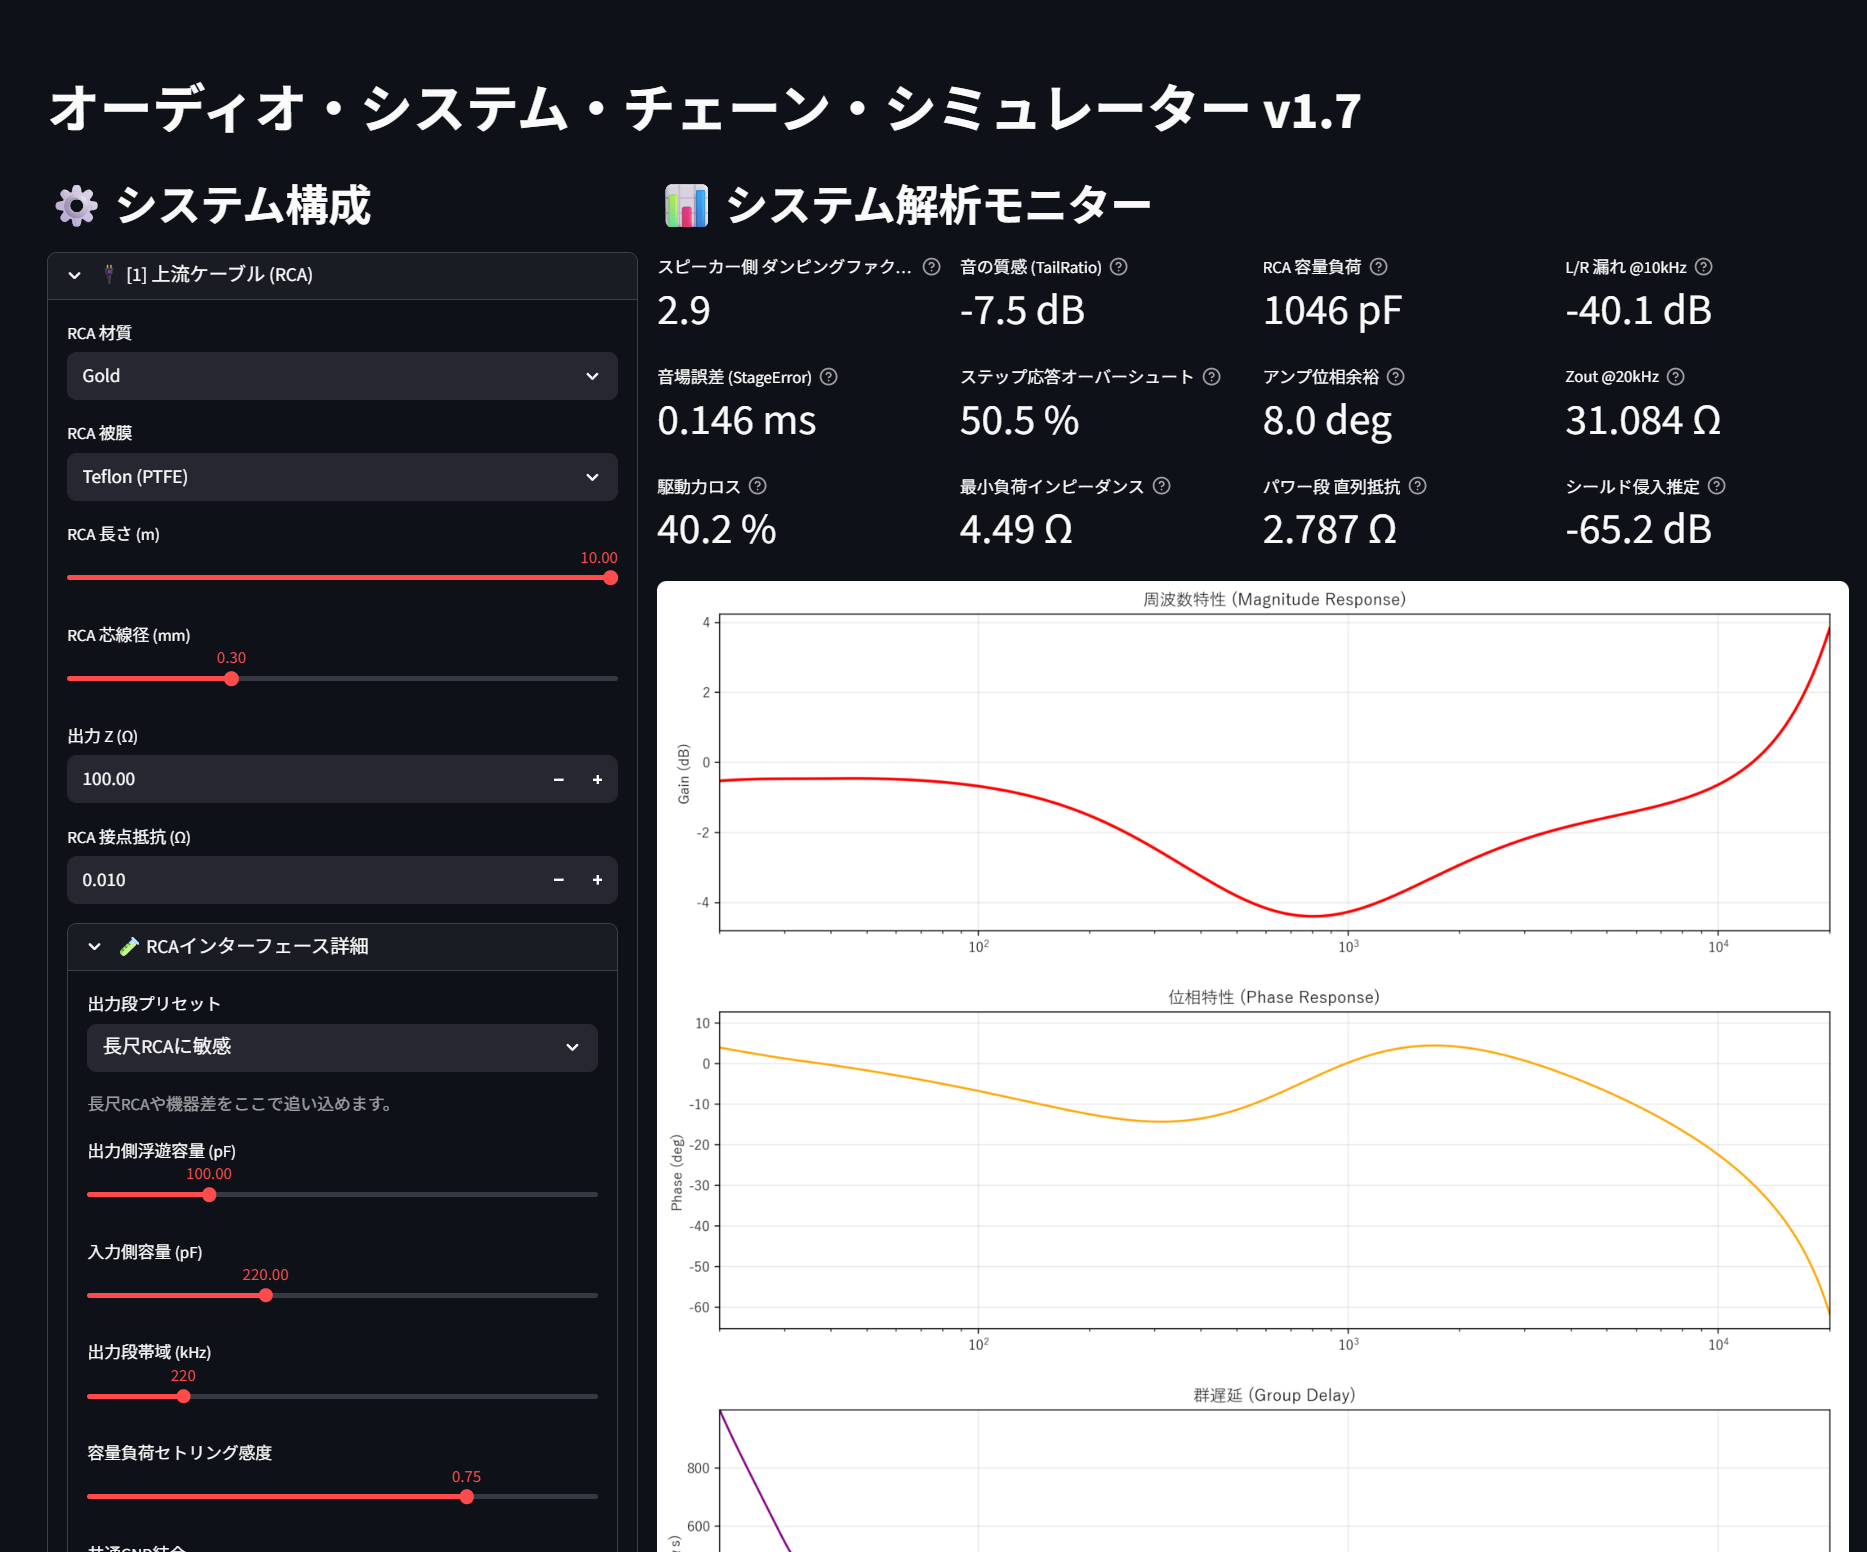
\includegraphics[width=\linewidth]{../../docs/images/app-screenshot.png}
  \caption{Current Streamlit application used for parameter control, analysis, and listening preview.}
  \label{fig:app-ui}
\end{figure}

\section{Model Components}

\subsection{Cable Model}

The cable model is RLGC-inspired and parameterized by conductor material,
geometry, dielectric type, contact resistance, and length. It exposes total
capacitance, total inductance, DC series resistance, return impedance, and a
frequency-domain transfer function.

\subsection{Interface Model}

The line-stage model includes source impedance, input impedance, parasitic
capacitance, settling behavior, common-return coupling, shield-quality stress,
and contact degradation estimates. This block is intended to model why a poor
or degraded RCA run may sound more veiled than a simple one-pole low-pass would
predict.

\subsection{Amplifier Models}

Two amplifier views are used.

\begin{itemize}
  \item A small-signal model estimates loop stress, pole shift, phase margin, and frequency-dependent output impedance.
  \item A nonlinear model applies slew-rate limitation, power sag, and harmonic generation.
\end{itemize}

Together, these blocks let cable and load parameters influence amplifier
behavior instead of assuming an ideal voltage source.

\subsection{Speaker Load Model}

A synthetic complex speaker-load model approximates resonance, inductive rise,
back-EMF-like behavior, and crossover-like branching. This is used to explain
why very long speaker-cable runs can sound less controlled or less forceful,
not merely quieter.

\subsection{Perceptual-Facing Metrics}

The framework reports:

\begin{itemize}
  \item TailRatio
  \item StageError
  \item damping factor
  \item drive loss
  \item crosstalk estimate
  \item shield-ingress estimate
  \item phase-margin estimate
  \item output impedance at 20 kHz
  \item impulse and step response features
\end{itemize}

These are not treated as proof of perception by themselves. They are treated as
bridges between physical/circuit changes and listening language.

\section{Current Results}

The current implementation already supports several qualitative findings.

\begin{itemize}
  \item Long or degraded RCA conditions can produce measurable HF attenuation, worsened tail behavior, and worse ingress/contact indicators.
  \item Very long speaker-cable conditions can reduce damping factor and increase drive-loss-related metrics.
  \item A complex load model produces more realistic ``loss of grip'' behavior than a simple resistive-inductive load alone.
  \item Under extreme conditions, the resulting degradation is easy to reproduce in a way that is perceptually understandable.
\end{itemize}

At the same time, the simulator does not yet reproduce the author's full
listening experience under conditions that feel sufficiently persuasive. In
particular, qualities such as veil, treble sheen, extension, soundstage shift,
and increased density remain only partially explained. These results should
therefore be interpreted as simulation findings, not yet as fully bench-validated
conclusions.

\section{Validation Plan}

The next validation steps should include:

\begin{enumerate}
  \item bench measurements with multiple RCA lengths and speaker-cable lengths
  \item square-wave or step-response comparison under varying capacitive load
  \item ablation studies isolating capacitance, shielding, and contact degradation
  \item measured impedance import for real speakers, headphones, or IEMs
  \item controlled listening studies where practical
\end{enumerate}

\section{Limitations}

The present implementation still has important limitations.

\begin{itemize}
  \item speaker loading is synthetic rather than measurement-driven
  \item RF ingress and hum are approximated, not modeled as full stochastic processes
  \item bad-contact behavior is a soft deterministic approximation
  \item real amplifier Bode measurements are not yet imported
  \item listening validation remains incomplete
\end{itemize}

These limitations are not side notes; they define the boundary of the current
claims.

\section{Conclusion}

This work introduces an integrated simulation framework for studying
cable-related degradation in audio systems at the level of the full signal
chain. The current conclusion is intentionally limited but meaningful.

The simulator can already reproduce, in a perceptually understandable way,
degradation caused by extreme operating conditions. This supports the practical
claim that audio quality can degrade when cables are used under sufficiently
poor conditions.

However, the author's own listening experience is not yet fully explained. In
particular, cable-related veil, treble sheen and extension, soundstage change,
and the impression of a denser sound have not yet been reproduced under
conditions that feel fully satisfactory. Those gaps are not failures to hide;
they are the clearest indication of where further research is required.

The value of the present work is therefore twofold. First, it replaces vague
debate with a structured model that can be inspected, extended, and measured.
Second, it clearly separates what has already been reproduced from what still
remains unresolved. For a first paper, that is already a meaningful and honest
result.

\section*{Acknowledgements}

The implementation and drafting process benefited from iterative development
assistance and technical discussion with ChatGPT and Gemini. These tools are
credited as development aids, not as scientific authors.

\end{document}

